\documentclass[
	%a4paper, % Use A4 paper size
	letterpaper, % Use US letter paper size
]{jdf}

\usepackage{graphicx}
\usepackage{subfig}
\usepackage{float}
\usepackage{adjustbox}


\author{
	Richard Albright \\
	903548616}
\email{ralbright7@gatech.edu}
\title{Project 6: Indicator Evaluation}

\begin{document}
%\lsstyle

\maketitle

\begin{abstract}
The development of a theoretically optimal portfolio strategy, and evaluation of indicators for later use in a machine learning algorithm.
\end{abstract}

\section{Introduction}
The project develops an theoretically optimal portfolio strategy as a sanity check for later machine learning algorithm use. Five indicators are also evaluated for later use in the same aforementioned machine learning algorithm.  The indicators picked are; simple moving average, exponential moving average, bollinger band percent, moving average convergence divergence, and momentum. 

\section{Theoretically Optimal Portfolio Strategy}

A theoretically optimal portfolio strategy would have perfect knowledge of future price movement.  Since the historical price data given is limited to daily prices, an optimal strategy would need to know upcoming price movement 1 day into the future.  With this knowledge in hand, the porftolio would be adjusted to be long or short at the current days price.  If the stock price was known to be higher the following day, the portfolio would enter a long position.  If the stock price was known to be lower the next day, the portfolio would enter a short position.  If the stock price was known to be unchanged the next day, the portfolio would continue to hold its current position, regardless if long or short.  

The constraints for this exercise assume no price impact due to the portfolio's trading or any  commissions incurred.  Starting cash is \$100,000. The simulation is based on trading JPM between January 1, 2008 and December 31, 2009.  Net Holdings are never being long more than 1000 shares, and never being short more than 1000 shares at any given time. This would mean the max trade can either long or short 2000 shares, in order swing from the maximum and minimum.  With these constraints in place, the optimal portfolio strategy will initially execute a 1000 share order either long or short, then either buy or sell 2000 shares to swing the total holdings to the maximum or the minimum shares allowed. For example, it the initial trade is to buy 1000 shares, this position will be held until the next days price is known to be less than the current days.  At that time, the portfolio would sell 2000 shares at the current day's close price, creating a short position of 1000 shares, knowing that the following day the closing price will be less than the current day's.  The short position would then be held until the next day's closing price was known to be higher than the current days closing price.  At that time, the portfolio would then buy 2000 shares, to flip the short position of 1000 shares to a long position of 1000 shares. We will compare this strategy to the benchmark of Buying 1000 shares of JPM and holding a long position for the entire period.

\begin{figure}[h]
	\begin{tabular}{c}
		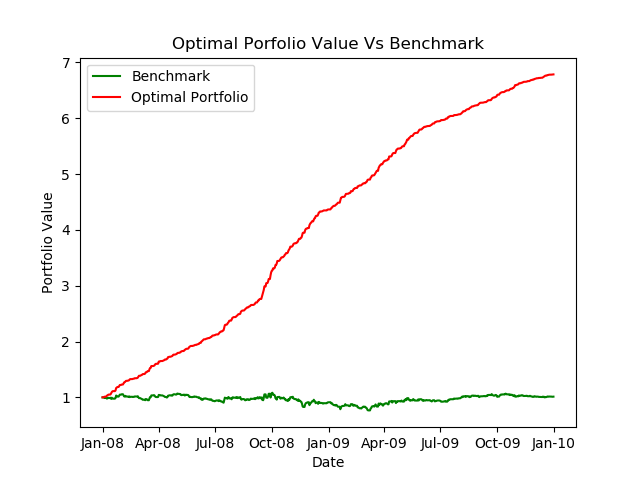
\includegraphics[height=10cm]{optimal_portfolio.png} \\
		\textbf{Figure 1} \\
	\end{tabular}
\end{figure}

Figure 1 represents the results of the execution of the Theoretically Optimal Portfolio Strategy.  Starting with an initial cash outlay of \$100,000, the optimal portfolio had an ending value of \$678,610, while the benchmark had an ending value of \$101,230.  

\pagebreak 

Below is a table of summary metrics of the Optimal Strategy vs the benchmark.

\begin{table}[h]
\centering
\begin{tabular}{ c | c | c}
  \hline
  Metric & Optimal Strategy & Benchmark \\
  \hline   
 
Cumulative Return & 5.7861 & 0.0123 \\
Mean of Daily Returns & 0.0026 & 0.0001 \\
Std Dev of Daily Returns & 0.0042 & 0.0141 \\
Sharpe Ratio & 10.0316 & 0.1304 \\
Ending Value & \$678,610 & \$101,230 \\
  \hline
\end{tabular}
\caption{Theoretically Optimal Portfolio Metrics}
\label{tbl:topic_overlap}
\end{table}

\section{Indicators}

\subsection{Simple Moving Average (SMA)}

A simple moving average is the simple (unweighted) mean over the last k points in a series. It can be represented as:

\begin{equation}
SMA_{k} = \frac{P_{1} + P_{2} + ... + P_{k}}{k} 
\end{equation}

where P equals a series of points, n = number of means calculated from the series over a window of k points.  The simple moving average can be a useful indicator of a price trend. A 200 day period is popular for indicating a long term trend, while a 50 day period is popular for indicating a short term trend. Simple moving averages can be combined and create trending indicators.  A shorter term SMA crossing over a longer term SMA on the upside is known as a golden cross indicator, indicating an possible uptrend.  A shorter term SMA crossing over a longer term on the downside is known as a death cross and indicates a possible downtrend. A short term SMA also smooths out volatility and can be used to reduce noise in the series. The simple moving average is a lagging indicator, and works well in determining areas of support and resistance. 

\pagebreak

Below is an image of JPM's 50 day simple moving average.

\begin{figure}[h]
	\begin{tabular}{c}
		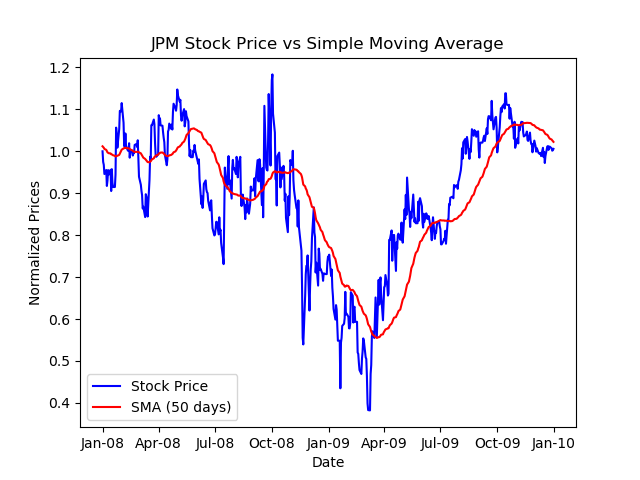
\includegraphics[height=10cm]{JPM_sma.png} \\
		\textbf{Figure 1} \\
	\end{tabular}
\end{figure}

\subsection{Exponential Moving Average (EMA)}

An exponential weighted moving average has a weighted mean over the last k points in a series.  The weights are determined by calculating the smoothing factor $ \alpha = \frac{2}{k+1}$ The weights for each point decline exponentially as we go back in time based upon the smoothing factor $ \alpha $.  The calculation for EMA then becomes:

\begin{equation}
EMA_{k} = \frac{P_{k}+(1-\alpha)P_{k-1}+(1-\alpha)^{2}P_{k-2}+...+(1-\alpha)^{k}P_{0}}{1+(1-\alpha)+(1-\alpha)^{2}+...+(1-\alpha)^{k}}  
\end{equation}

The exponential moving average can be used similarly to the simple moving average.  Since the exponential moving is weighted more heavily with more recent prices, the average is more responsive to price shifts than the simple moving average. Like the simple moving average, the can also be used to smooth volatility and can be used as a substitute for raw prices when reducing noise of a signal.

\pagebreak
Below is an image of JPM stock price vs a 5 day exponential moving average, note the reduction of volatility vs the daily prices.
\begin{figure}[h]
	\begin{tabular}{c}
		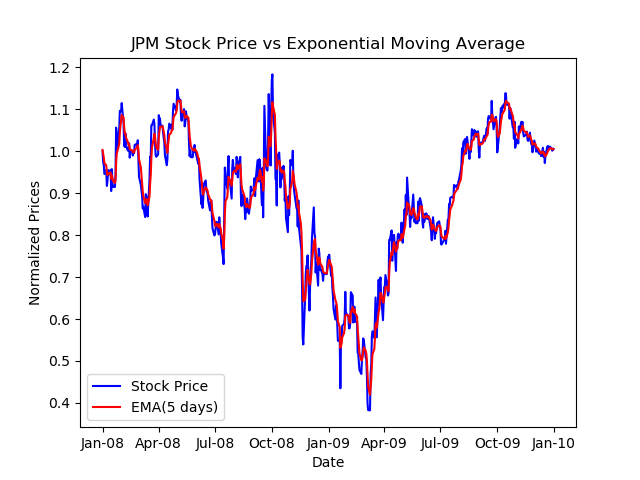
\includegraphics[height=10cm]{JPM_ema.png} \\
		\textbf{Figure 2} \\
	\end{tabular}
\end{figure}

\subsection{Bollinger Band Percent}

The bollinger band percent indicator is a variant of bollinger bands that plots the stock price in percentage terms in relation to the higher and lower bands.  To calculate bollinger bands, an envelope of upper and lower bands are created above and below the mean (MA) of historical prices (P) for a given period k.  These bands are calculated (BOLU - upper, BOLD - lower) )by adding or subtracting a given standard deviation ($\sigma$) level (m) from the mean.  Which can be calculated as:

$ BOLU = MA(P, k) + m \sigma(P, k) $

$ BOLD = MA(P, k) - m \sigma(P, k) $

$ BBP = \frac{P - BOLD}{BOLU - BOLD} $

This indicator can be used for determining if a stock is trading above or below its historical average. A score of 0.5 is trading at the moving average. A score >= 1 means the price is at least m standard deviations above the moving average, a score <= 0 means the price is at least m standard deviations below the moving average. A mean reversion strategy could be run with this lagging indicator, going long the stock at a score <= 0, and short the stock >= 1, then close out the position when crossing the mean at 0.5.

The image below is JPM's Stock Price vs a 50 Day Bollinger Band.  The percentage is using a 5 day exponential moving average in substitution for the price in order to smooth the signal. 

\begin{figure}[h]
	\begin{tabular}{c}
		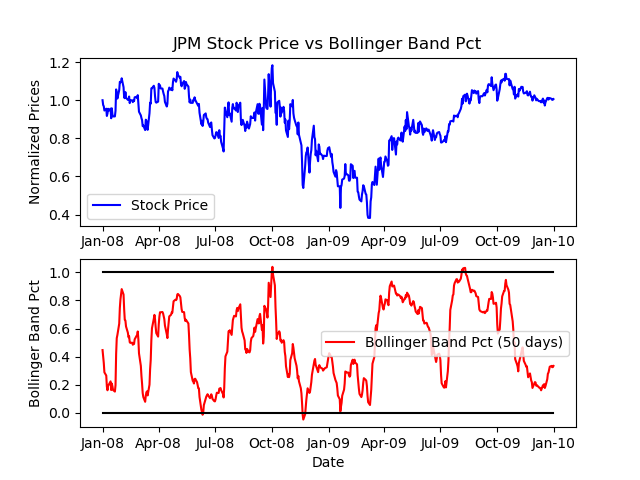
\includegraphics[height=10cm]{JPM_bollinger.png} \\
		\textbf{Figure 3} \\ 
	\end{tabular}
\end{figure}


\subsection{Moving Average Convergence Divergence (MACD)}

The moving average convergence divergence indicator is a momentum indicator that uses subtracts a fast exponential moving average (f - shorter period) from a slow exponential moving average (s - longer period).  This number is then also smoothed with an exponential moving average used as a signal. Convergence is indicated as the fast and slow averages approach each other, and divergence is indicated when the averages drift apart from each other. The formula for MACD can be represented as 

MACD = EMA(P, s) - EMA(P, f) 

MACD signal = EMA(MACD, k)

signal line = MACD - MACD signal

where k is some smoothing factor in days.  A pretty common MACD implementation uses 12 periods for f, 26 periods for s and 9 periods for k.  To use MACD as an indicator, if the signal crosses to above 0, this is a long signal.  If the signal to crosses below 0 this is a short signal. The image below shows JPM's stock price vs MACD using the aforementioned default periods, plotting a signal line crossover.


\begin{figure}[h]
	\begin{tabular}{c}
		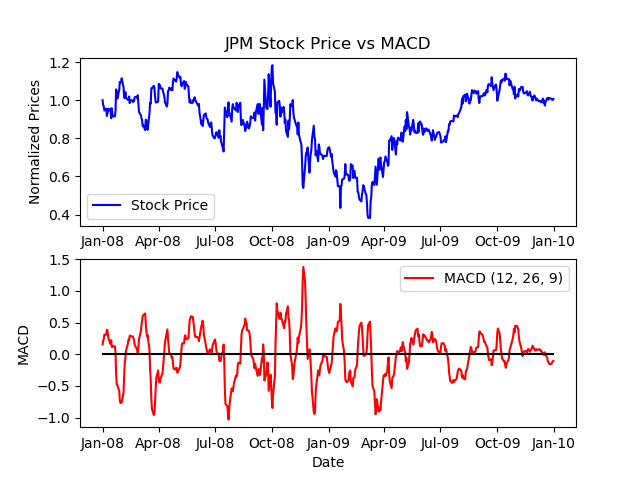
\includegraphics[height=10cm]{JPM_macd.png} \\
		\textbf{Figure 4} \\ 
	\end{tabular}
\end{figure}


\subsection{Momentum}

The momentum indicator represents the percent change in a price on day k vs a prior price n days ago.  It can be derived as follows:

Momentum = $ \frac{P_{k}}{P_{k-n}} - 1 $

A mean reversion strategy could be used here, If the momentum indicator crosses an upper bound then take a short position, if the momentum indicator crosses a lower bound then take a long position.

The image below displays JPM's stock price vs a 20 day momentum indicator, using a +-20\% signal threshold.


\begin{figure}[h]
	\begin{tabular}{c}
		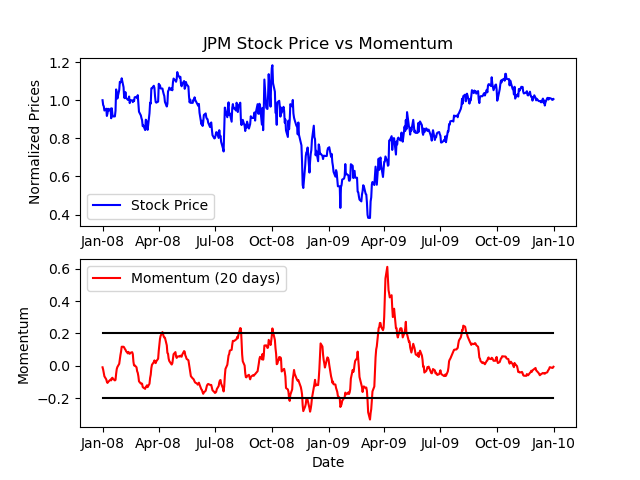
\includegraphics[height=10cm]{JPM_mom.png} \\
		\textbf{Figure 5} \\ 
	\end{tabular}
\end{figure}

\makeatletter
\renewcommand\@biblabel[1]{\textbullet}
\makeatother

\begin{thebibliography}{shortest-entry}

\bibitem{Wikipedia} Wikipedia \textit{Moving Average}, \url{https://en.wikipedia.org/wiki/Moving\_average}, 2021
\bibitem{PyData} PyData \textit{pandas.DataFrame.ewm}, \url{https://pandas.pydata.org/docs/reference/api/pandas.DataFrame.ewm.html}, 2021
\bibitem{Investopedia} Investopedia \textit{Bollinger Band Definition}, \url{https://www.investopedia.com/terms/b/bollingerbands.asp}, 2021
\bibitem{Wikipedia} Wikipedia \textit{MACD}, \url{https://en.wikipedia.org/wiki/MACD}, 2021

\end{thebibliography}

\end{document}